% begin Chapter ProposedSolution

\chapter {Gaman: A solution prototype}
\label{chapter-SolutionPrototype}

\paragraph {} So far we have seen how the problem of the public transport system is structured and how it affects the stakeholders. We also saw how the nature of the problem demands a Decision Support System-like solution. This Chapter provides details about the solution prototype, titled "Gaman", that was built for the purposes of this research project. The architecture of the system is provided along with the system features. The Chapter ends with a few UI screenshots of the prototype that was developed to test the usability and effectiveness of the functionality with the users.

\section{System Architecture}

\paragraph{ } Gaman is designed as a web application following the client-server model. This design is the most conducive to the problem as it enables access to all stakeholders concerned in a distributed fashion. Therefore, commuters can access the system on-demand while allowing the schedulers access to the system and the data in real-time.

The solution prototype used the three-tier architecture in the application. This architecture was chosen because it allowed the development of the prototype to be faster and more easily adaptable to possible requirements changes. The technologies used for Gaman are listed below,

\begin {itemize}
\item Programming Language: PHP
\item Database: MySQL
\item Versioning System: GitHub
\item UI Framework: Twitter Bootstrap
\item Theme: Flatly theme by Bootswatch (Source: http://bootswatch.com/2/flatly/)
\end {itemize}

The software architecture of the system is depicted in Figure~\ref{image-gamanSystemArchitecture}.

\begin {figure} [H]
\centering
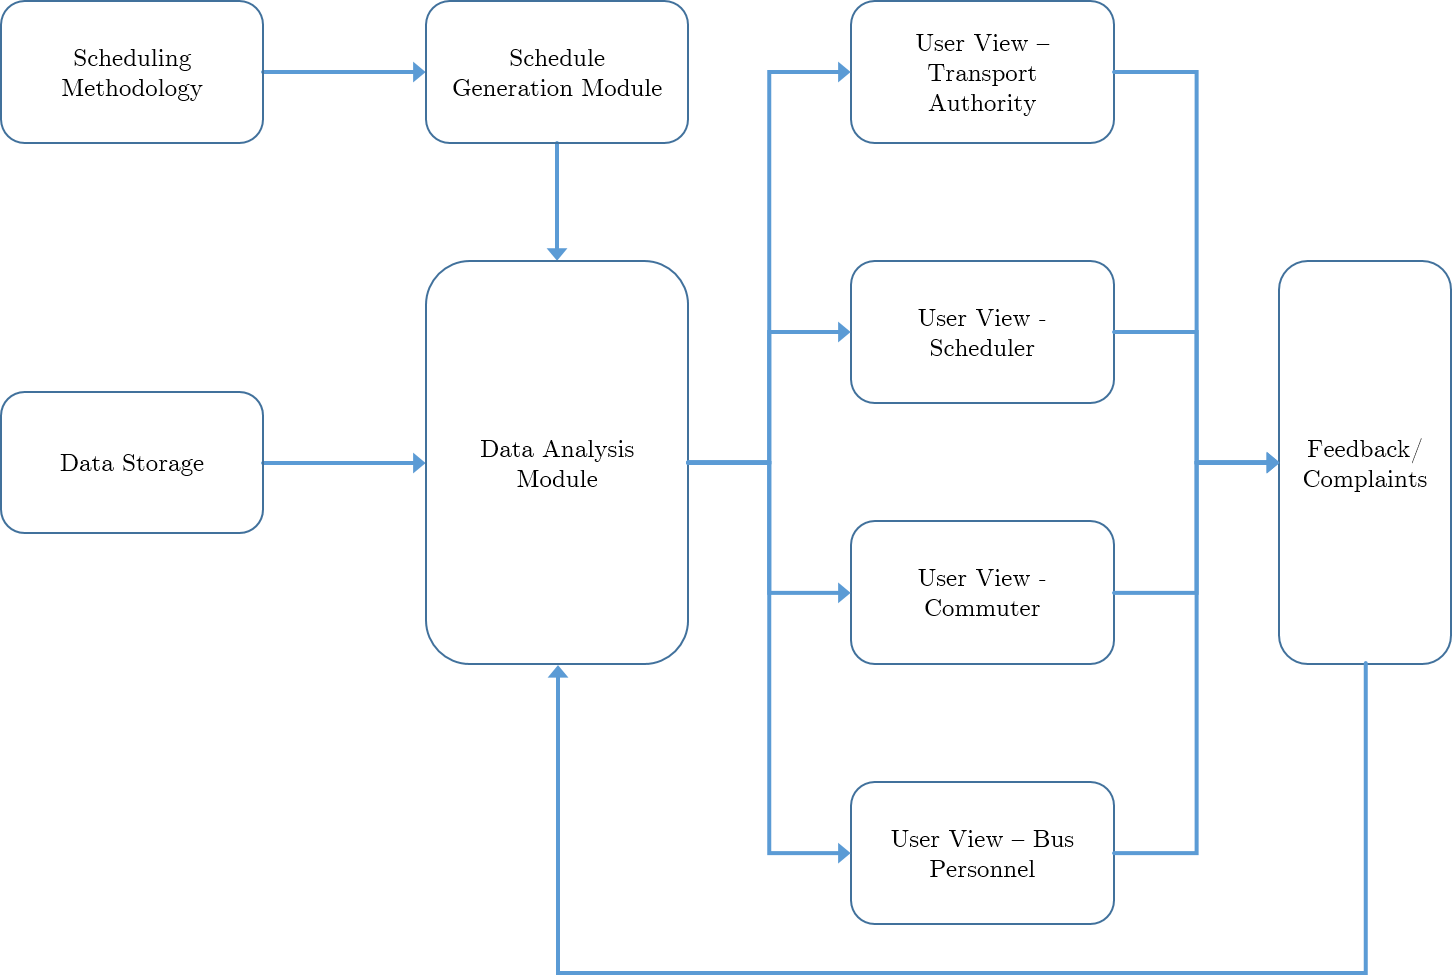
\includegraphics [scale=0.5] {gamanSystemArchitecture}
\caption [Proposed System Architecture] {Proposed System Architecture}
\label {image-gamanSystemArchitecture}
\end {figure}

The prototype that was created only included a subset of this whole architecture due to time and resource constraints. Specifically the Scheduling Methodology unit and the Schedule Generation module was not included due to the above mentioned project limitations. 

\subsection{System users} 

\paragraph{} The system is designed with the "Commuters", "Schedulers", "Bus Personnel" and "Transport Authority" (other transport authority personnel) as their core users. The "Schedulers" act as the main Admin role in the system and they have the permission to manipulate all entities and functions of the system.  The role of "Transport Authority" is also defined as an Admin role but only provided to other personnel at the transport authority such as higher management personnel, training and development officers etc.

Separate user views have been provided for the "Commuters" and the "Bus Personnel". "Bus Personnel" refers to the owners and the operators of the buses together. The way the current bus system is structured, ownership of the buses is with third party private owners instead of the transport authority or the government. Therefore it is important to make the distincttion between the users and provide separate views for them.

\subsection{System Entities \& their Relationships}

\paragraph{} The Proposed System works with 4 main entities at it's core. They are,

\begin {itemize}
\item \textbf{Bus Routes} - Bus Routes refer to the routes that the buses provide the service on. They consist of a Beginning Bus Stop, an Ending Bus Stop and Bus Stops in between. One Bus Route may have many Stops
\item \textbf{Bus Stops} - This refers to the place allocated for a Bus to stop and drop off and/or pick up passengers. This is also known as the Bus Stand
\item \textbf{Buses} - This refers to the individual Buses that operate and provide the service to the commuters. One Bus is assigned to only one Bus Route. One Bus may have many Bus Personnel attached to it.
\item \textbf{Bus Personnel} - This refers to the people involved with the operation of the buses. This includes the Bus Driver, the Bus Conductor and the Bus Owner. In certain instances, these roles overlap. Accordingly, there may be situations where a Bus Driver is also an Owner or a Bus Conductor who is also an Owner. Each Bus Person (singular of Personnel) is assigned to only one Bus.
\end {itemize}

\paragraph{} Apart from these 4 core entities, the \textbf{Complaints} and the \textbf{General Feedback} entities are present. They exist to provide much needed feedback to the schedulers so that service quality can be maintained. These entities provide the basis for the Feedback step in the timetabling process of the schedulers (For more information regarding this process, see Figure~\ref{image-timetablingProcessSteps}).

Additionally the \textbf{Survey}, \textbf{Trip} and \textbf{Stop Activity} entities exist to aid the Survey functionality of the schedulers. A brief intro into what these entities are is listed below,

\begin {itemize}
\item \textbf{Survey} - An investigation of the buses in a route in terms of the passenger loads on the buses plying on that route. These are called route surveys and the Schedulers say ascertain the passenger loads as input for the timetabling through this process. One Survey is conducted on only one route at a time.
\item \textbf{Trip} - A trip is one-way journey between the Beginning Stop and the Ending Stop of a Bus Route. A Survey has many Trips included. Within the Trip, there are many Stops, and consequently many Stop Activities.
\item \textbf{Stop Activity} - A Stop Activity is the record of the exchanges of passengers that occurs at a Bus Stop during a Trip. 4 main facts are recorded for a Stop Activity when the bus stops at a Bus Stop. The number of passengers who get off the bus, number of people that get on the bus, the time (timestamp) the bus came to a stop and the passengers started to get off the bus at the Bus Stop and finally the time (timestamp) the bus departed the Bus Stop.
\end {itemize}

The above mentioned entities allow the Schedulers to carry out a route survey and gather the necessary data for the timetabling process. The Route Surveys that the Schedulers perform are imperative in their timetable formulation as it acts as the data input for the process. The Schedulers mainly obtain the Passenger Load information which is directly related to the dispatching of buses on a route. Loiter time data is also used to identify errant bus operators as well as to continuously monitor the total travel time on a route.



\section{System Features}
\label{systemFeatures}

\paragraph{ } The list of system features and functionality is noted below. Please note, the features marked under \textit{Public} is available for the regular commuters to access while the functionality marked under \textit{Admin} is only available for the Schedulers and other administrative staff at the Transport Authority.

\begin{itemize}

\item Public Functions
\begin{itemize}
\item \textbf{Information Portal for Bus Routes, Stops, Buses and Bus Personnel} - This is, as its name suggests, the functionality of providing the data about the 4 main entities related to the transportation service in a smile easy-to-use, easy-to-read-and-understand interface. The information includes the basics from name of stop (for Bus Stops) and the Stops along a particular route (for Bus Routes) to more advanced things like the Personnel assigned to a particular Bus and the number of complaints received on a particular Bus.
\item \textbf{Information Portal for Bus Fares} - This would basically provide the details of the Bus fares in a given route.
\item \textbf{Bus Route Finder functionality} - When an origin and destination stop are given, the user is presented with a list of bus routes to take
\item \textbf{Submitting and reviewing submitted General Feedback} - Using this functionality, users can provide comments (good or bad) regarding the 4 main entities. This goes hand in hand with the Complaints and acts as a complimenting function to the Complaints.
\item \textbf{Submitting and reviewing submitted Complaints} - Users can submit their complaints to the authority and these will be investigated and action taken. The Complaints also acts as a notification for the Schedulers in their timetabling process. For instance when there are a lot of complaints on a particular route regarding overcrowded buses or consistently delayed buses, the Schedulers can reconsider the timetable for that route and improve it. Currently this connection between the Complaints and the Schedulers is not available and therefore the Schedulers have no idea which areas need improvement.
\end{itemize}

\item Admin Functions
\begin{itemize}
\item \textbf{Survey data storage, retrieval and visualization} - this is one of the main functionalities of the proposed system. it provides the knowledge base as well as the main input to the timetabling process of the Schedulers.
\item \textbf{Timetable Storage, Retrieval and Visualization} - Timetables are documents that the buses are dispatched according to. The tracking of buses according to their dispatch times is currently done manually. The times that the buses are dispatched are recorded on timetable and sent in to the regional offices. This functionality of the system attempts to digitize that by having a digital representation of the data so that it can be stored and retrieved later.
\item \textbf{Timetable Generation} - This functionality enables the schedulers to automatically generate timetables for a given route. As mentioned previously, this is currently done manually and the proposed system would incorporate a the feature of generating the timetable by calculating the average headways.
\item \textbf{Vehicle and Crew Scheduling} - This is the next step in the planning process. The Vehicle and Crew Scheduling functions are the rosters that the bus operators follow. This function enables the Schedulers to automatically generate these without having to do this step of the process manually.
\item \textbf{Complaint and General Feedback tracking Dashboard} - The Complaint and General Feedback functions serve as the indicator in this system. It tells the Schedulers which routes are doing well and which ones aren't, which buses are breaking the law and which bus personnel has a good record. It allows the authority to analyze the quality of the service and includes the commuters in the process of measuring service quality.
\end{itemize}

\end{itemize}



\section{URL of prototype system}

\paragraph{} The prototype system can be found at the following URL: \url{http://gaman.byethost4.com/}. The system's Admin Interface can be found at \url{http://gaman.byethost4.com/admin/}. The login credentials for both these interfaces are listed below.

\begin{table} [H]
\centering
\begin{tabular}{|c|c|c|c|c|}
\hline
Area &username &password &First Name &Last Name \\
\hline
Public	&heisenberg	&123	&Walter	&White \\
\hline
Public	&whysoserious	&123	&The	&Joker \\
\hline
Public	&adopted	&123	&Loki	&Laufeyson \\
\hline
Public	&manofirony	&123	&Tony	&Stark \\
\hline
Admin	&admin	&123	&Admin	&User \\
\hline
\end{tabular}
\caption{Login Credentials - Gaman}
\label{table-loginCredentials}
\end{table}

\begin {itemize}

\item Public Area
\begin {itemize}
\item Username: \textbf{heisenberg}
\item Password: \textbf{123}
\end {itemize}

\item Admin area
\begin {itemize}
\item Username: \textbf{admin}
\item Password: \textbf{123}
\end {itemize}

\end {itemize}

The system is an active project on GitHub. The code repository can be found at, \url{https://github.com/afthaj/Gaman/}



\section{UI Screenshots}

\paragraph{} UI Screenshots of the prototype system are displayed below. The interfae has been kept as minimal as possible with only the required items being displayed so as not to deviate away from the users experience.

\begin {figure} [H]
\centering
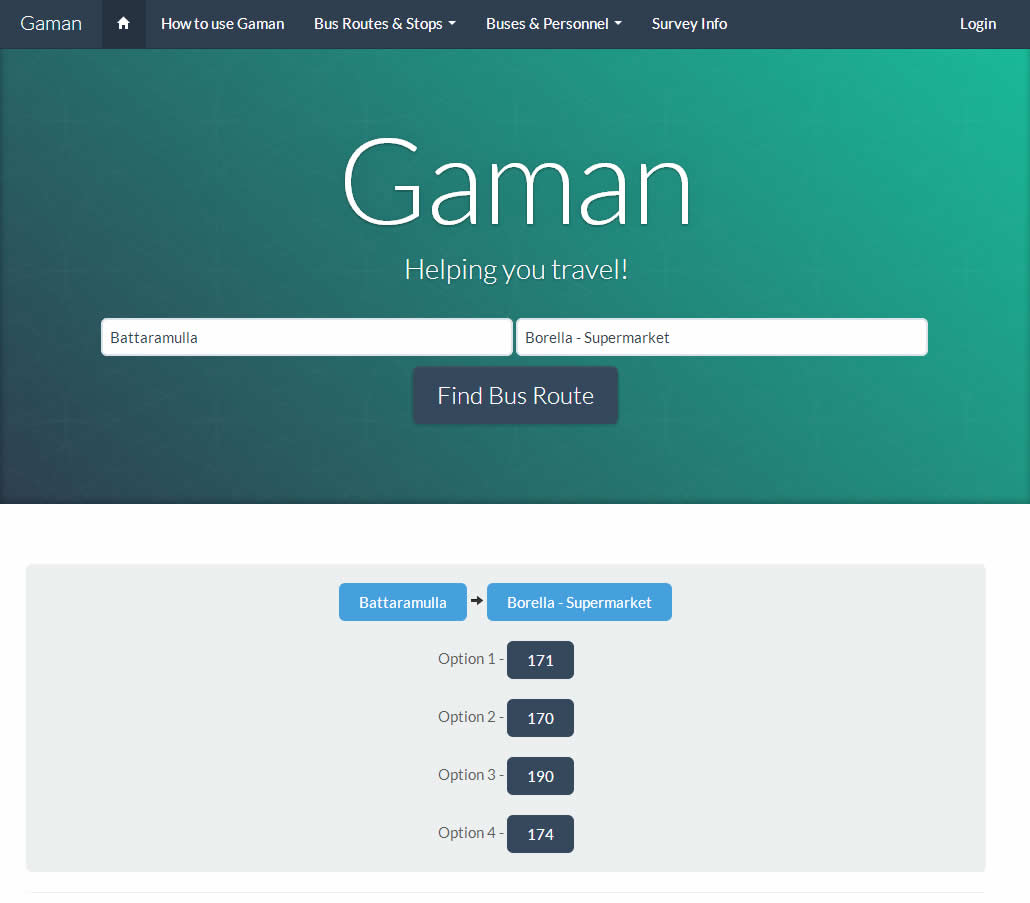
\includegraphics[scale=0.45]{public-home}
\caption [Screenshot - Public Home Page] {Screenshot - Public Home Page}
\label {image-public-home}
\end {figure}

\paragraph{} The home page of the public view of Gaman is displayed in Figure~\ref{image-public-home}. The front page contains the bus route finder so that users can input the origin and destination of their trip and find a suitable bus route directly from the home page. The links in the results area (shown in Figure~\ref{image-public-home}) are clickable so that users can click them directly for more information. This accesses the database and provides the users with information in a timely and accurate manner.

\begin {figure} [H]
\centering
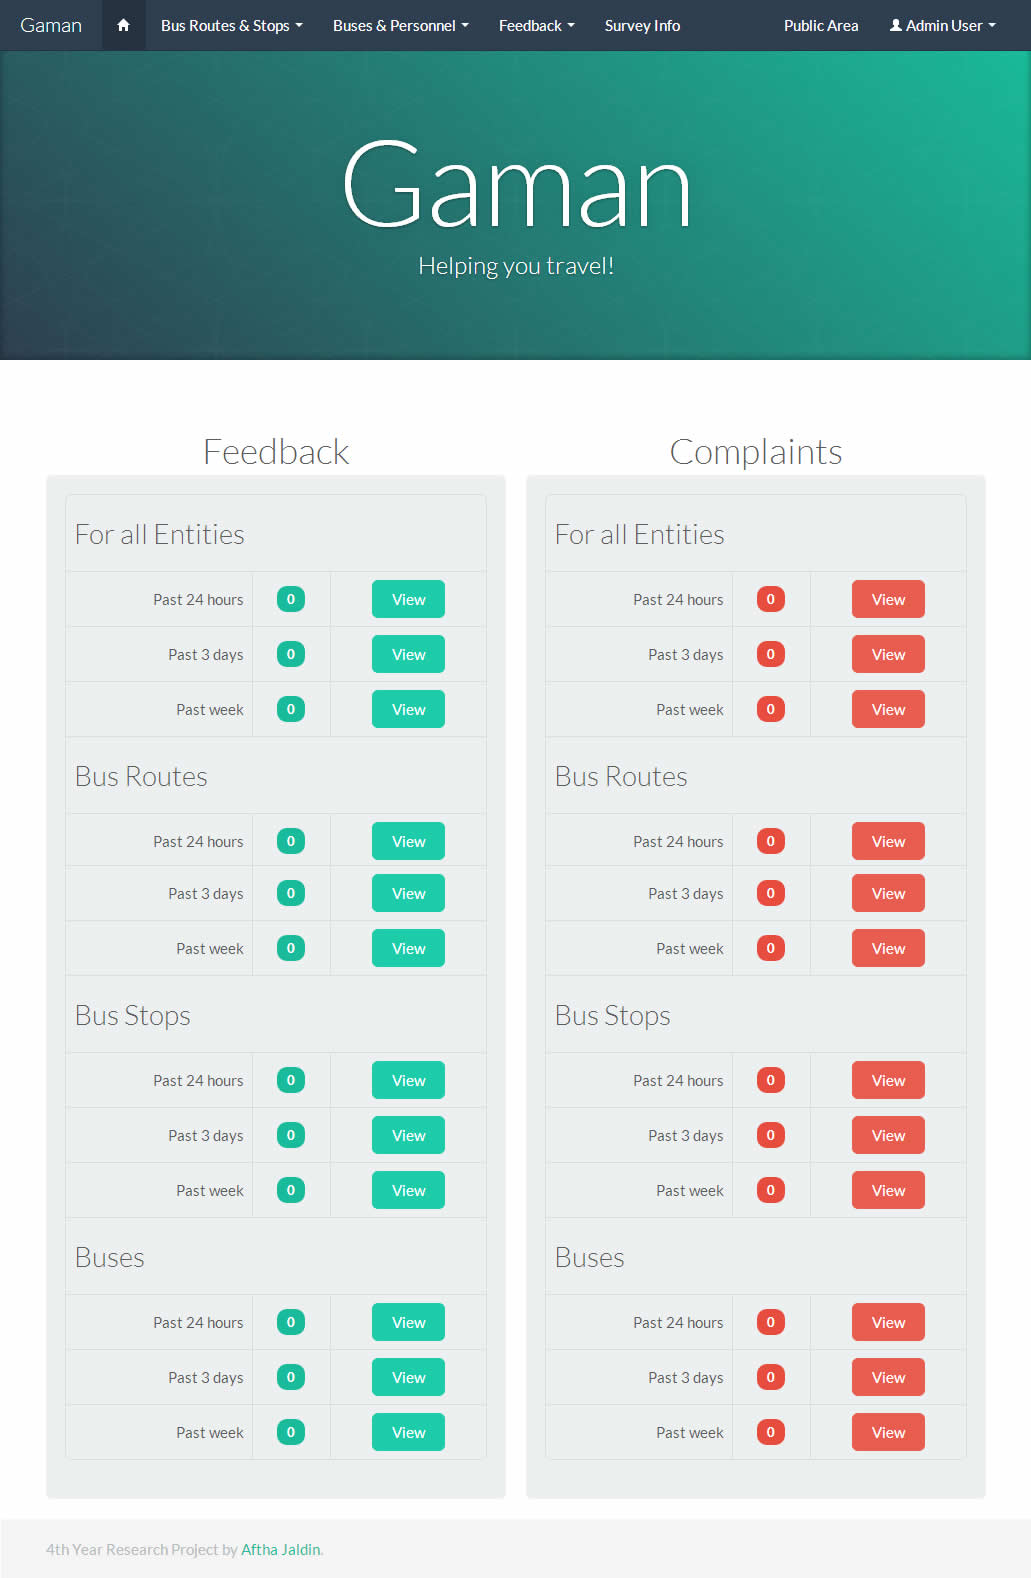
\includegraphics[scale=0.35]{admin-home}
\caption [Screenshot - Admin Home Page] {Screenshot - Admin Home Page}
\label {image-admin-home}
\end {figure}

\paragraph{} Figure~\ref{image-admin-home} shows the Home page of the admin users. it provides a dashboard view of the feedback and complaints that are received. This allows the schedulers to gauge the level of service currently in the bus service. Whenever these numbers increase, the schedulers will be alerted that an iunvestigation needs to be made and possibly a revision to an existing route timetable. These links too are clickable so that the users can navigate easily within the system.

\begin {figure} [H]
\centering
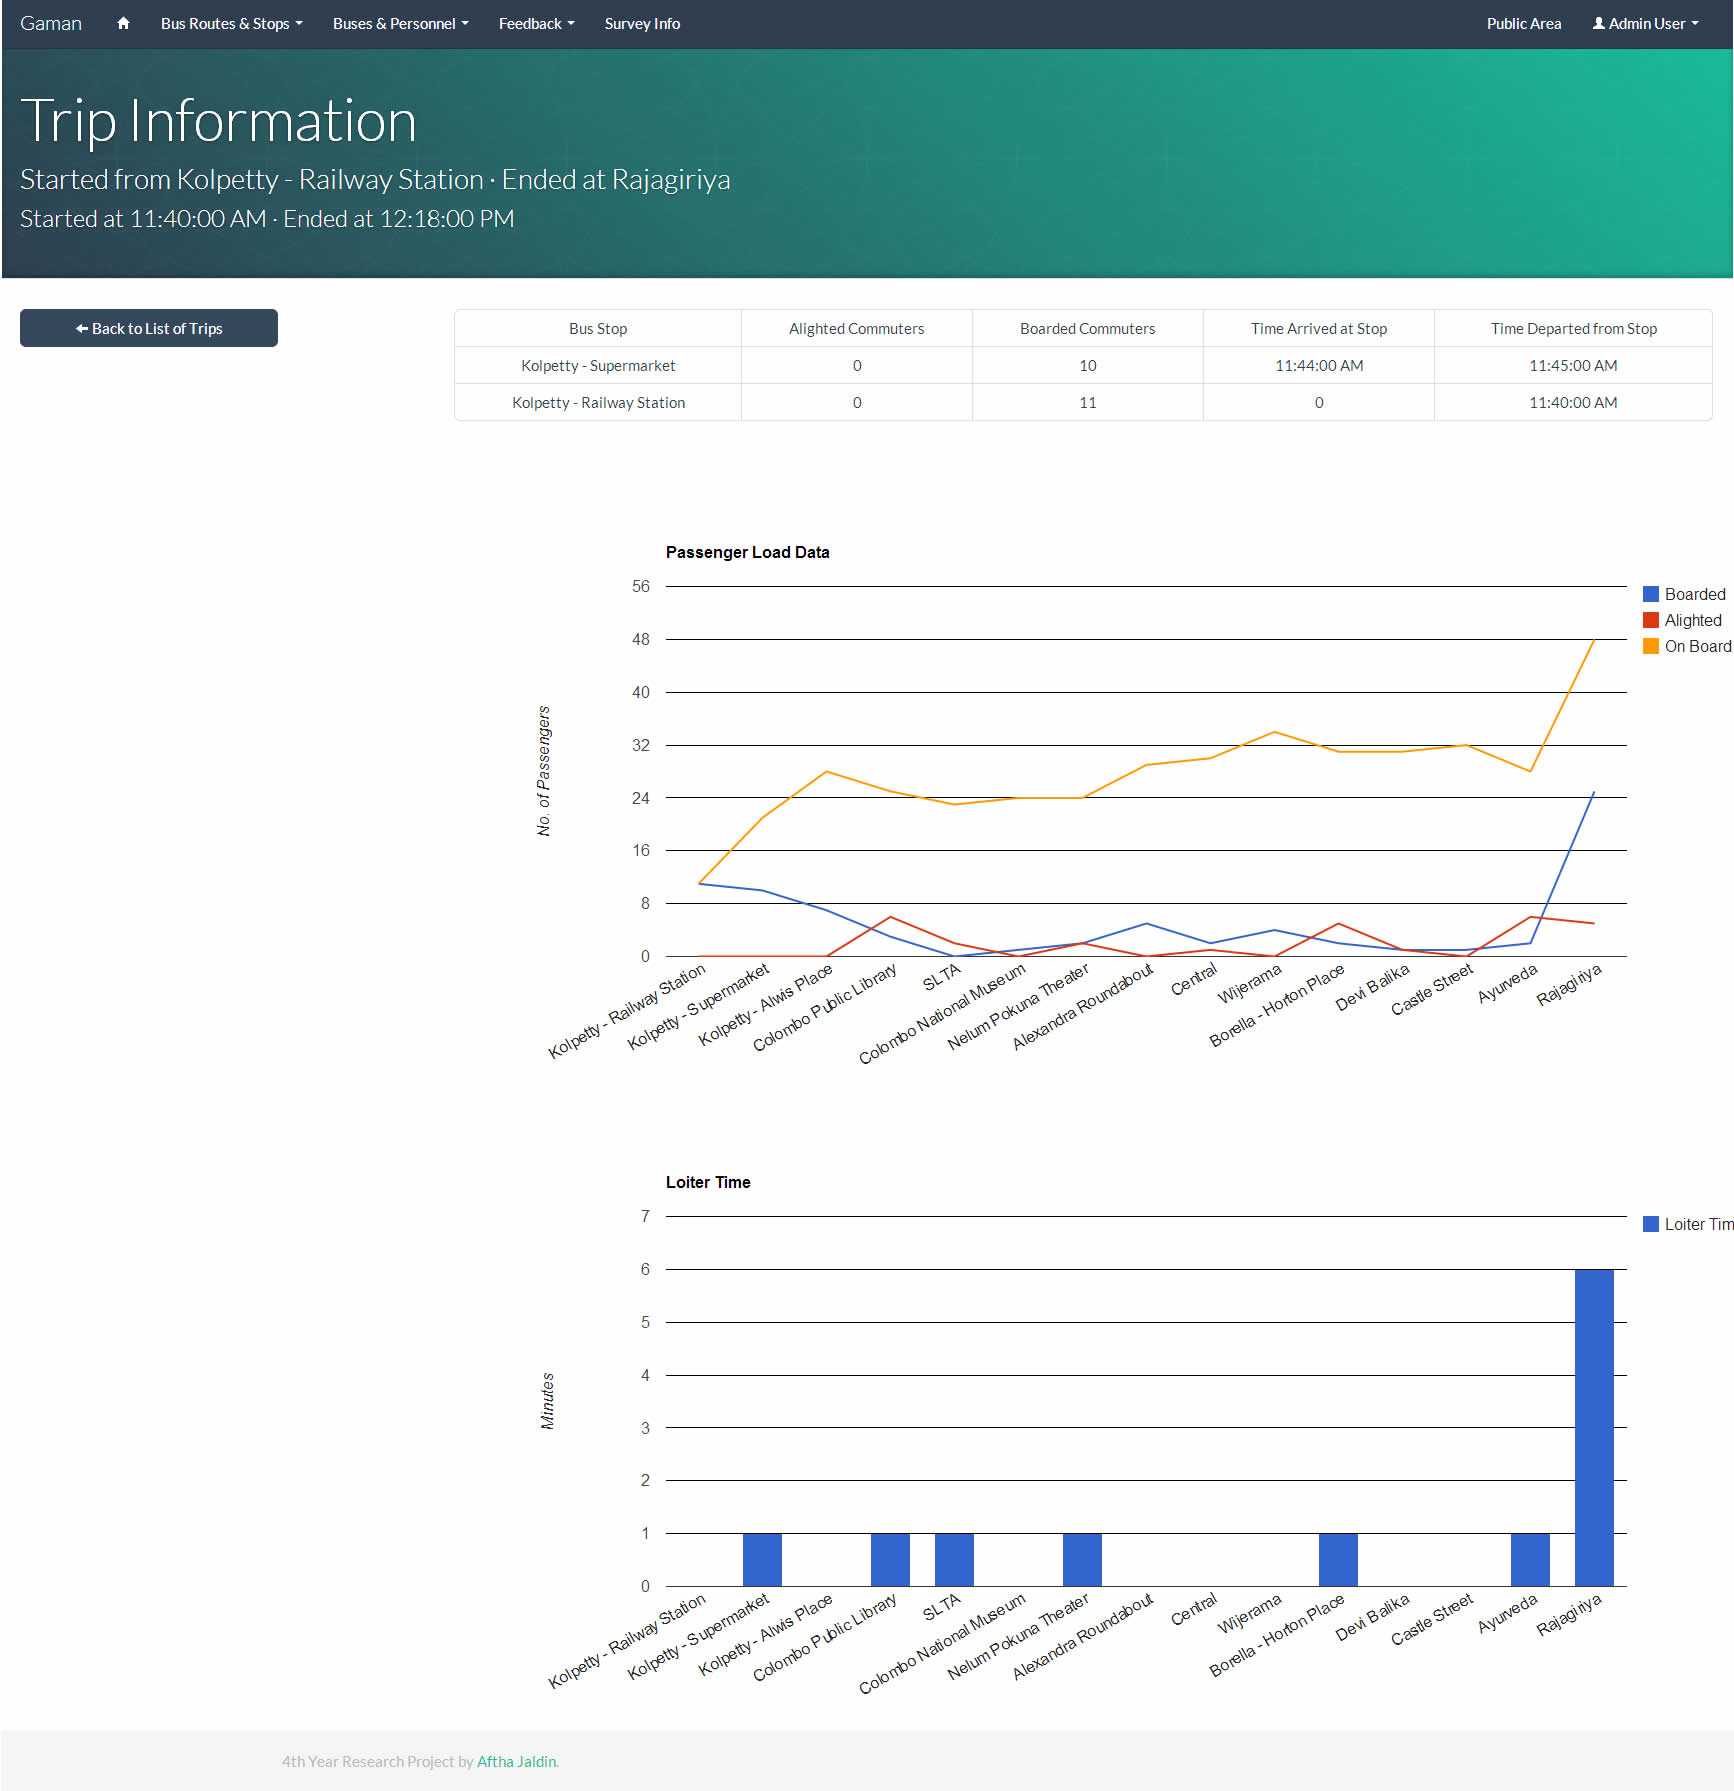
\includegraphics[scale=0.25]{admin-trip-information}
\caption [Screenshot - Survey Trip information] {Screenshot - Survey Trip information}
\label {image-admin-trip-information}
\end {figure}

\paragraph{} Figure~\ref{image-admin-trip-information} shows the user interface of the page where details of a trip in a given survey are displayed. Survey's are the primary source of input for the schedulers in their workflow and the display and analysis of the survey data is very important. This is why the data is visualized in this manner so that it aids the schedulers in their decision making process. By looking at it in a graphical form, schedulers can quickly gauge which areas need to improve and take steps accordingly.

\begin {figure} [H]
\centering
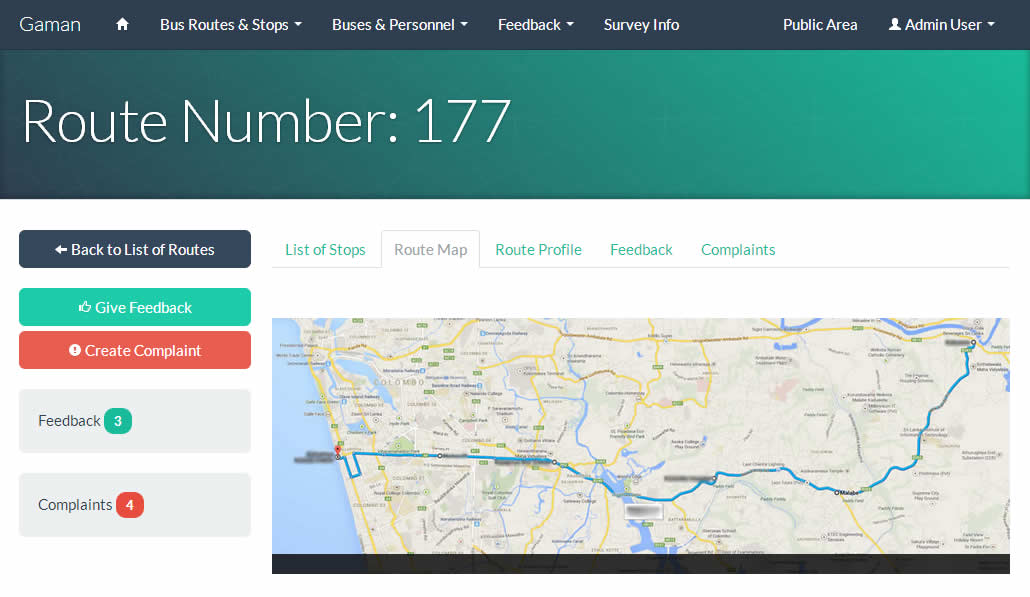
\includegraphics[scale=0.45]{admin-view-route}
\caption [Screenshot - View Route Details - Route Map] {Screenshot - View Route Details - Route Map}
\label {image-admin-view-route}
\end {figure}

\paragraph{} The inteface that shows the details of a given route is shown is Figure~\ref{image-admin-view-route}. The content on the View Route Details page consists of multiple tabs so that users can easily view the various details of the route without navigating to a sepratae page altogether. Figure~\ref{image-admin-view-route-2} and ~\ref{image-admin-view-route-3} also show the details in seprate tabs in the inteface. Figure~\ref{image-admin-view-route} shows the route and its stops on a map.

\begin {figure} [H]
\centering
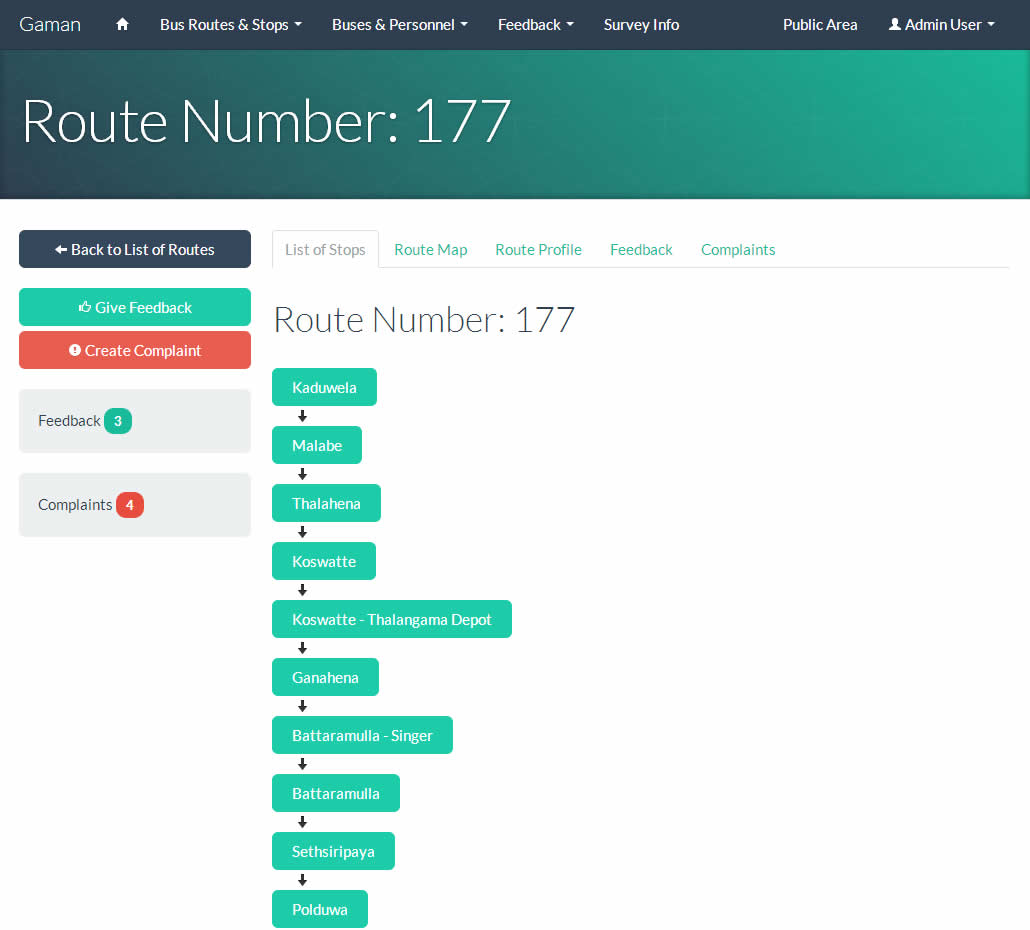
\includegraphics[scale=0.45]{admin-view-route-2}
\caption [Screenshot - View Route Details - List of Stops] {Screenshot - View Route Details - List of Stops}
\label {image-admin-view-route-2}
\end {figure}

\paragraph{} Figure~\ref{image-admin-view-route-2} shows the various bus stops on the route and the order that they are followed. Again, the names of these bus stops are clickable making navigation easier for the user. When clicked, it navigates the user to the page of the respective bus stop. The interface of that page is given by Figure~\ref{image-admin-view-stop}  later on in this chapter.

\begin {figure} [H]
\centering
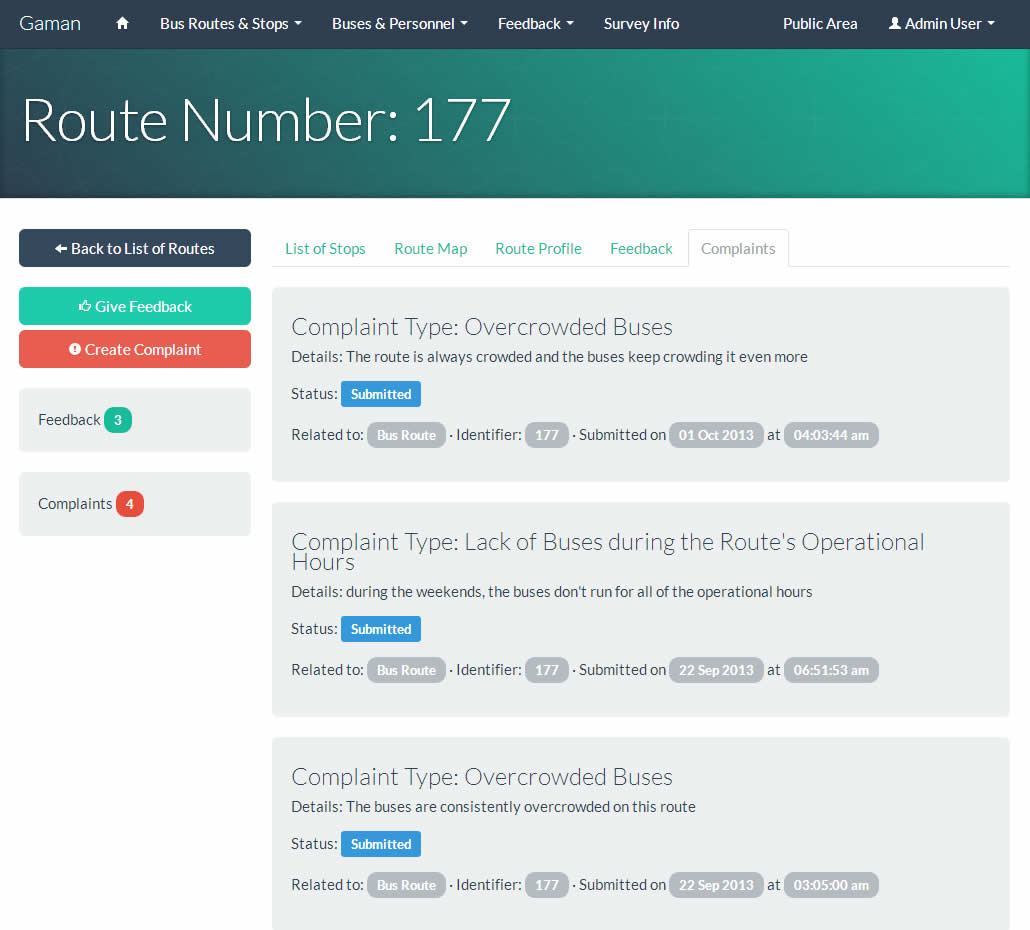
\includegraphics[scale=0.45]{admin-view-route-3}
\caption [Screenshot - View Route Details - Complaints] {Screenshot - View Route Details - Complaints}
\label {image-admin-view-route-3}
\end {figure}

\paragraph{} Figure~\ref{image-admin-view-route-3} shows the interface where the list of complaints received on that particular route are displayed. This is connected to the complaints and feedback functionalities of the system and displays information to the users that will allow them to choose a proper route for their journeys. Admins can also use this to gain a qualitative analysis of the present state of the route in terms of its feedback from the users.

\begin {figure} [H]
\centering
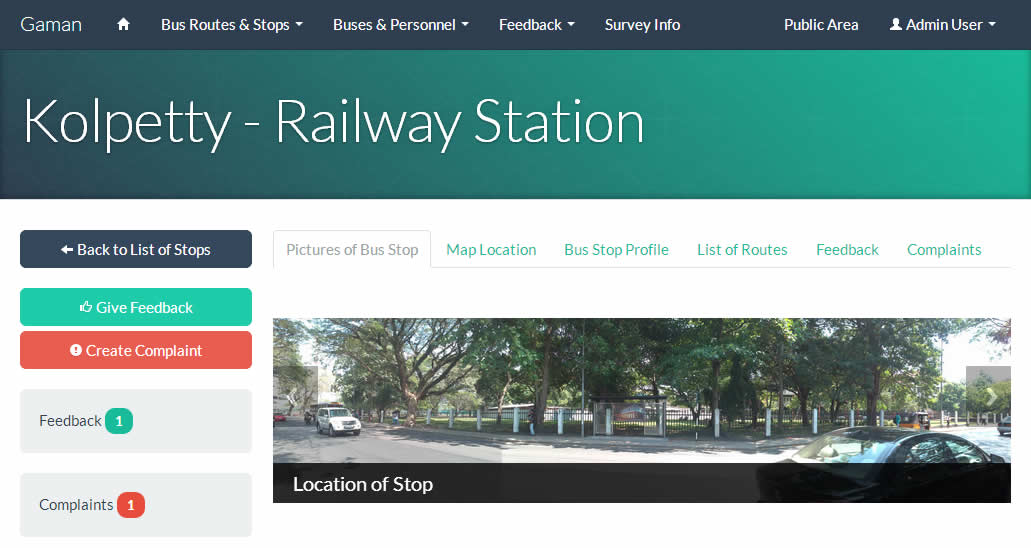
\includegraphics[scale=0.45]{admin-view-stop}
\caption [Screenshot - View Bus Stop Details - Panorama of stop location] {Screenshot - View Bus Stop Details - Panorama of stop location}
\label {image-admin-view-stop}
\end {figure}

\paragraph{} Figure~\ref{image-admin-view-stop} shows the interface for the page for viewing details about a given bus stop. This page again uses the tabbed interface so that the various details of the bus stops are provided to the users in a structured and organised manner. A panoramic view of the bus stop's location is provided so that users can identify where the bus stop is from the surrounding lankdmarks.

\begin {figure} [H]
\centering
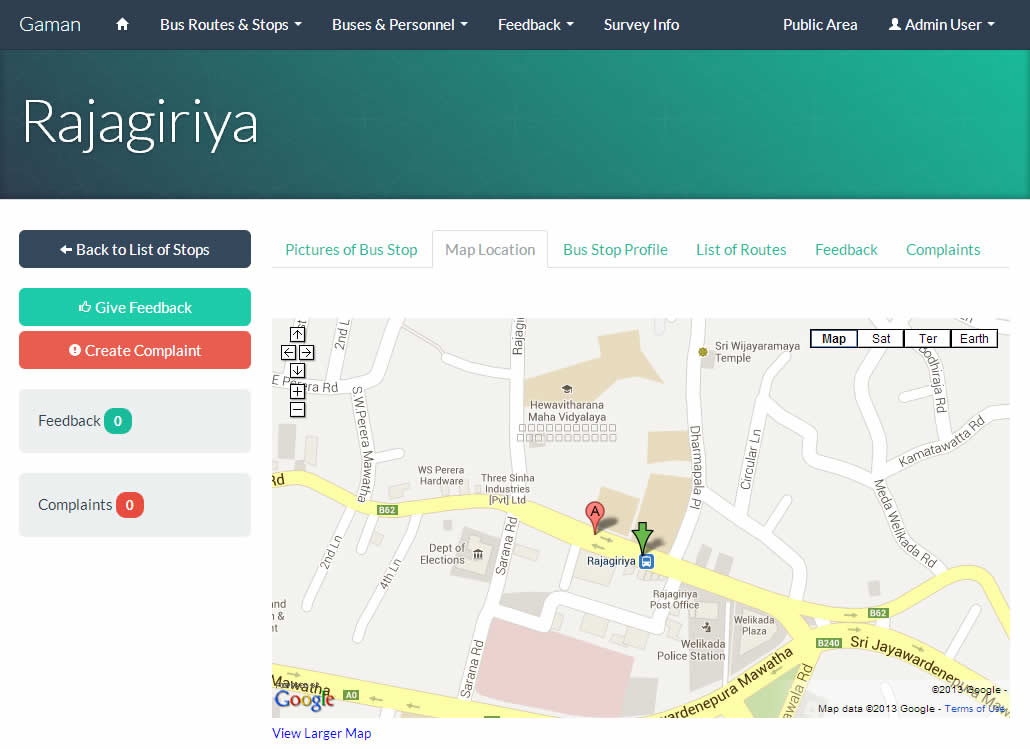
\includegraphics[scale=0.35]{admin-view-stop-2}
\caption [Screenshot - View Bus Stop Details - Location of stop on a map] {Screenshot - View Bus Stop Details - Location of stop on a map}
\label {image-admin-view-stop-2}
\end {figure}

\paragraph{} Figure~\ref{image-admin-view-stop-2} is a screenshot of another of the tabs in the page that users are provided to view the details about a certain bus stop. This tab shows the location of the bus stop on a map. 

\begin {figure} [H]
\centering
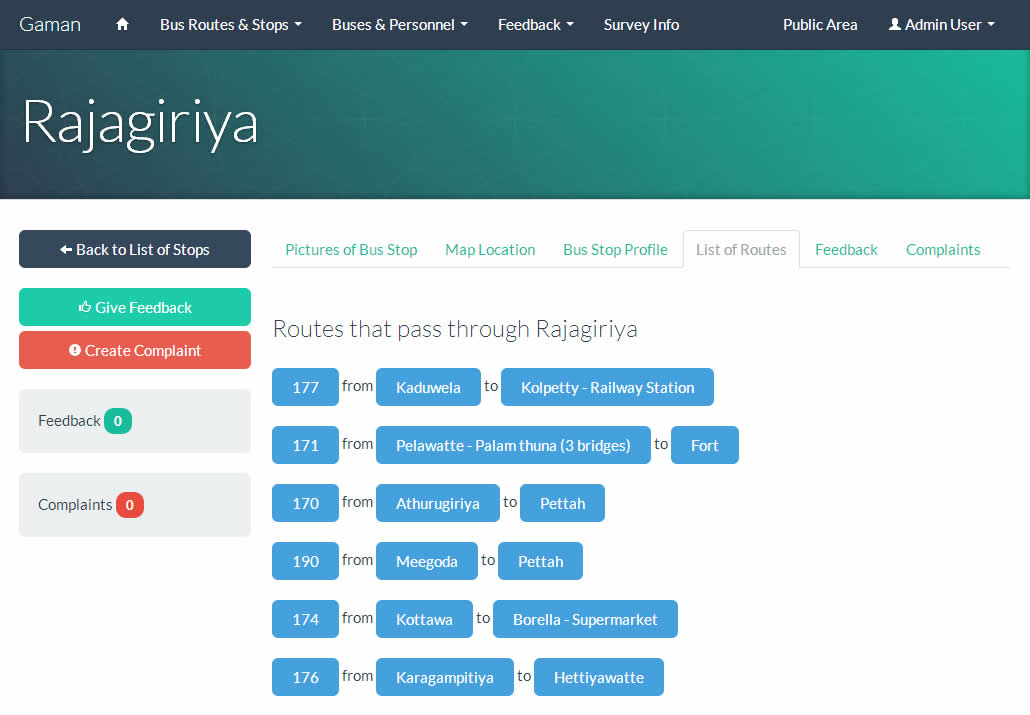
\includegraphics[scale=0.45]{admin-view-stop-3}
\caption [Screenshot - View Bus Stop Details - Routes that pass through bus stop] {Screenshot - View Bus Stop Details - Routes that pass through bus stop}
\label {image-admin-view-stop-3}
\end {figure}

\paragraph{} The tab that displays the list of routes that pass through a particular bus stop is shown in Figure~\ref{image-admin-view-stop-3}. This is important to note as it is a very helpful feature for the users. Commuters sometimes just want to know which bus routes pass through a particular bus stop and that information is provided in this tab. Similar to the previous pages and tabs, the routes and bus stops in this tab are clickable making navigation easier for the users.

This page also contains tabs for the list of Feedback items as well as the Complaints received for the particular bus stop. After logging in, users can view these and possibly add their own, thereby providing feedback to the schedulers and the transport authority to make the service better.

\begin {figure} [H]
\centering
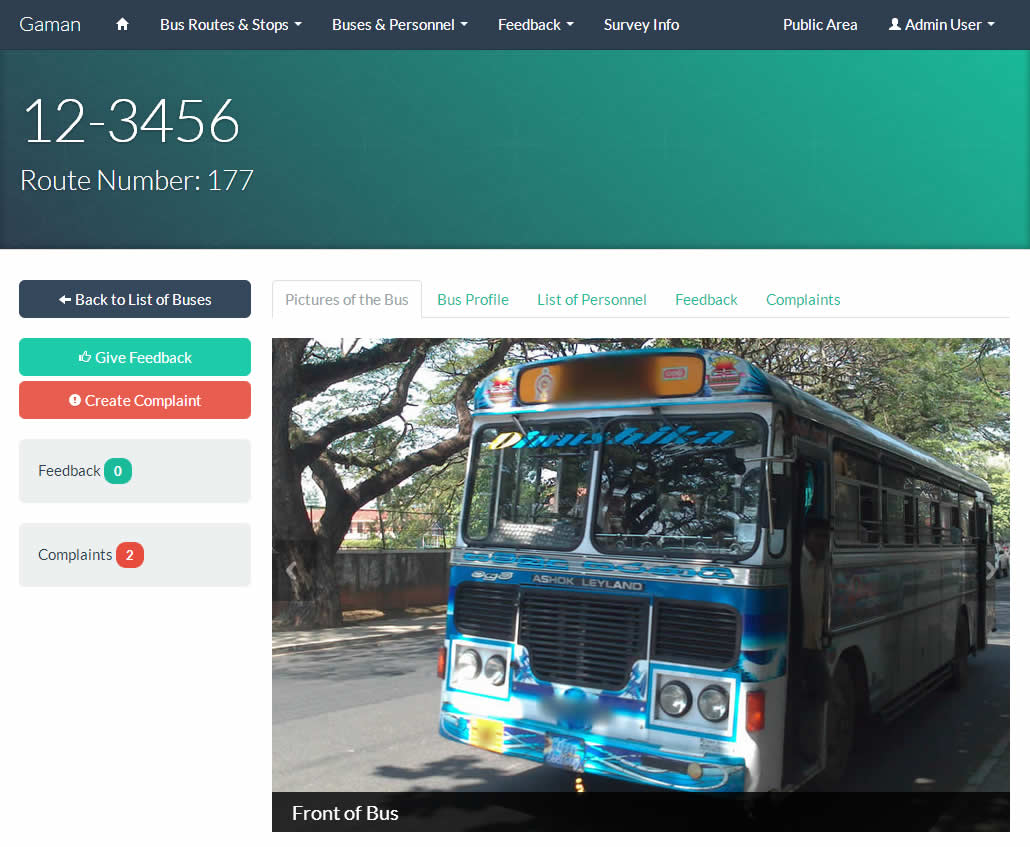
\includegraphics[scale=0.45]{admin-view-bus}
\caption [Screenshot - View Bus Details - Picture of Bus] {Screenshot - View Bus Details - Picture of Bus}
\label {image-admin-view-bus}
\end {figure}

\paragraph{} Figure~\ref{image-admin-view-bus} shows the page where users can view the details of an individual bus. Following the previous UI convention, this page too uses the tabbed interface to provide users with a clean organised look to the information while providing all the information in one single page. Pictures of the bus are provided in one of the tabs so that users can identify the bus exactly. Information provided in other tabs include the bus profile, list of personnel attached to a bus and the list of feedback and complaints.

\begin {figure} [H]
\centering
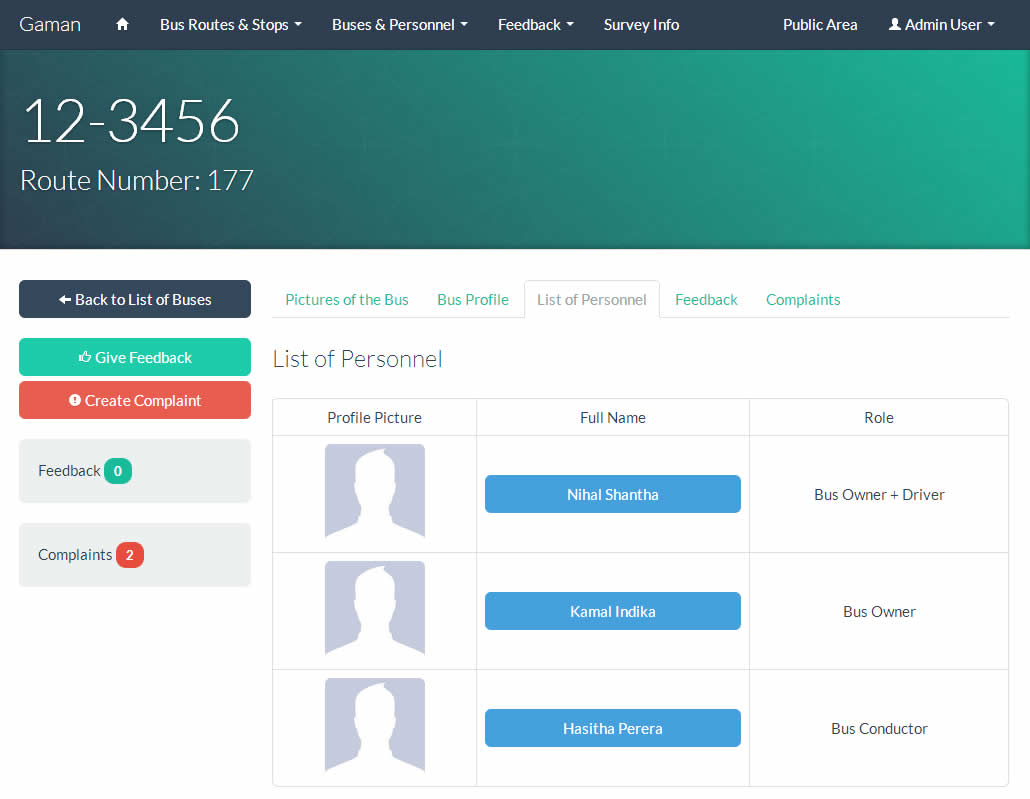
\includegraphics[scale=0.45]{admin-view-bus-2}
\caption [Screenshot - View Bus Details - List of Personnel of Bus] {Screenshot - View Bus Details - List of Personnel of Bus}
\label {image-admin-view-bus-2}
\end {figure}

\paragraph{} As mentioned previously, the page to view the details of an individual bus are given in Figure~\ref{image-admin-view-bus-2}. In this tab, the list of bus personnel attached to a bus (the bus owner, the driver, the conductor etc.) can be viewed by the user. Following the previous convention, the names of personnel can be clicked. the user will then be navigated to the respective bus personnel's details page. Again, this has been doen to improve navigation within the system for the users.

\begin {figure} [H]
\centering
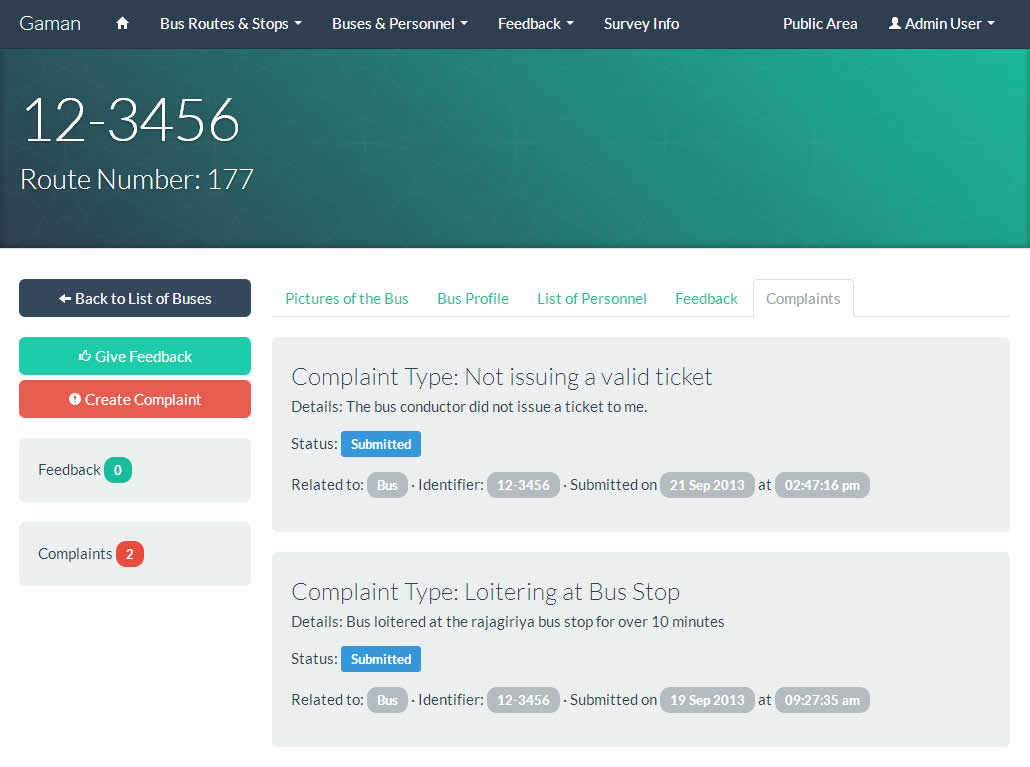
\includegraphics[scale=0.3]{admin-view-bus-3}
\caption [Screenshot - View Bus Details - List of Complaints of Bus] {Screenshot - View Bus Details - List of Complaints of Bus}
\label {image-admin-view-bus-3}
\end {figure}

\paragraph{} Figure~\ref{image-admin-view-bus-3} shows the UI for the tab that shows the list of complaints recieved on a particular bus. This again is helpful to the commuters as well as the schedulers to identify errant drivers and operators who behave in an unprofessional manner. Figure~\ref{image-admin-view-bus-personnel}shows the page that displays the details of individual bus persons (owner, driver, conductor etc.). Following the previous convention, this page also uses the tabbed interface and feature buses and bus routes that can be clicked to navigate to its respective details page.

\begin {figure} [H]
\centering
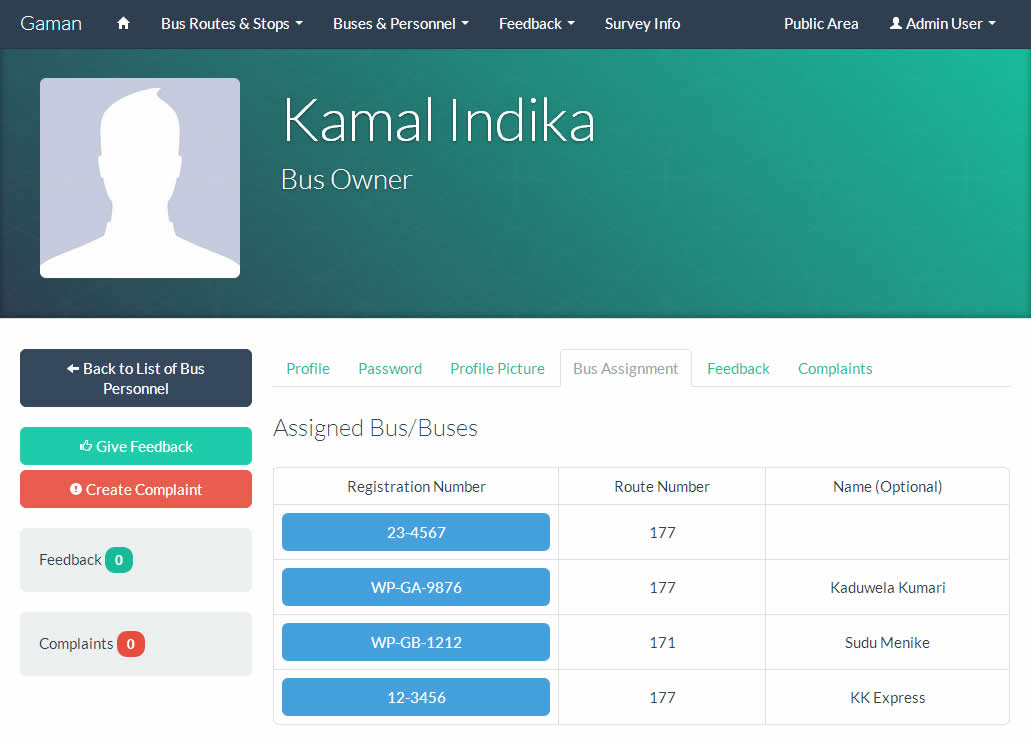
\includegraphics[scale=0.3]{admin-view-bus-personnel}
\caption [Screenshot - View Bus Personnel Details] {Screenshot - View Bus Personnel Details}
\label {image-admin-view-bus-personnel}
\end {figure}

\begin {figure} [H]
\centering
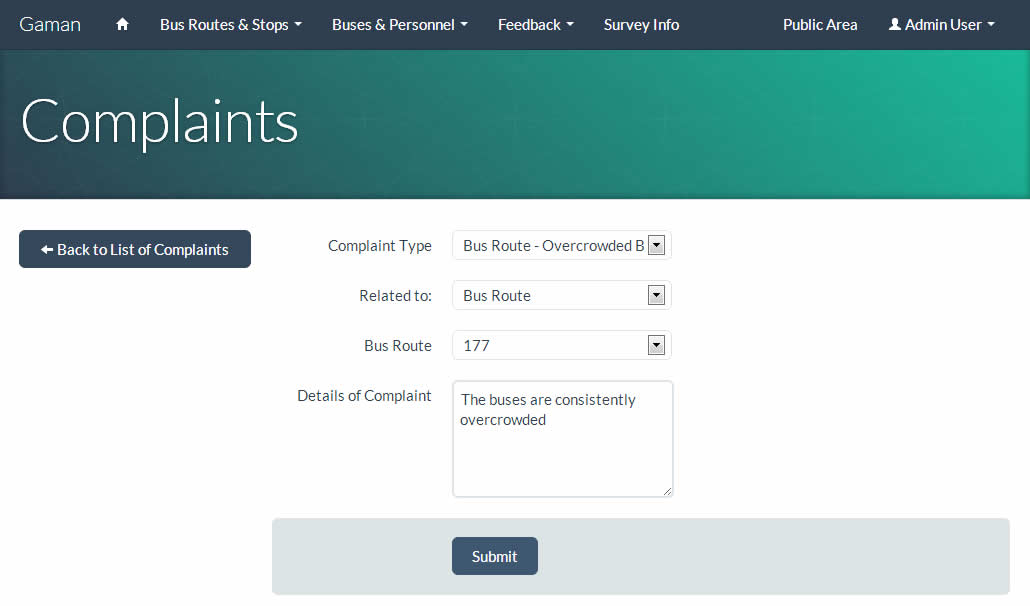
\includegraphics[scale=0.4]{admin-add-complaint}
\caption [Screenshot - Adding a new Complaint] {Screenshot - Adding a new Complaint}
\label {image-admin-add-complaint}
\end {figure}

\begin {figure} [H]
\centering
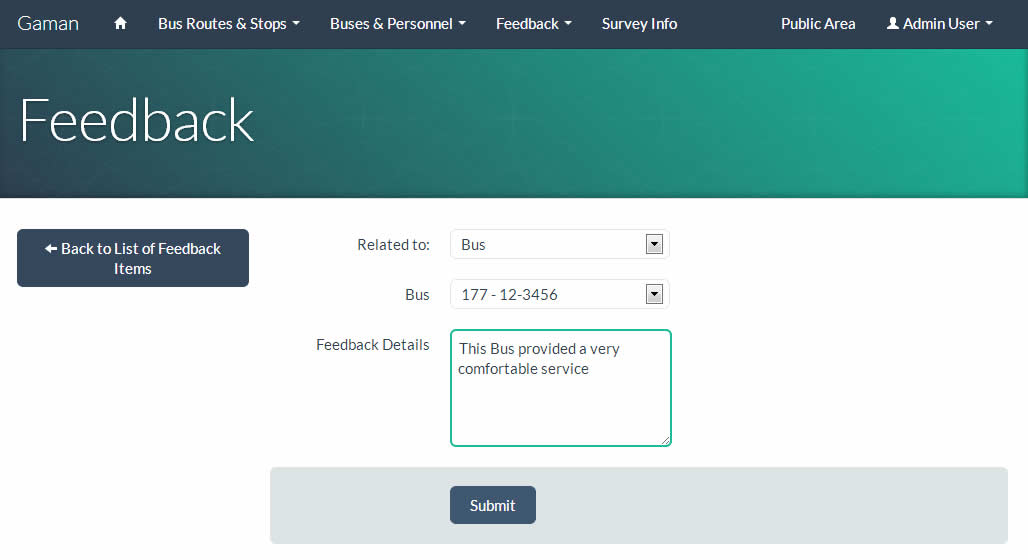
\includegraphics[scale=0.4]{admin-add-feedback}
\caption [Screenshot - Adding a new Feedback item] {Screenshot - Adding a new Feedback item}
\label {image-admin-add-feedback}
\end {figure}

\paragraph{} Figures~\ref{image-admin-add-complaint} and ~\ref{image-admin-add-feedback} show the UI of the page that allows the users to add a complaint or a feedback item. Users can choose from the relevant dropdown options and submit the complaint or feedback item. 

Dropdown options include but are not limited to,
\begin{itemize}
\item Bus Delays
\item Overcrowded Buses
\item Loitering at Bus Stop
\item Not issuing a valid ticket
\item Reckless driving
\item Neglecting road rules
\item Overcharging a bus fare
\item Rude/discourteous service
\item Unhygienic/non-presentable appearance and/or attire
\end{itemize}

Admin users can expand this list in the future. When a complaint type is chosen, the system automatically displays the list of related objects. For instance, if a complaint type related to bus routes is chosen, all the bus routes are shown in the follwoing dropdown menu for the user to choose from. This improves usability and prevents complaints being filed under the wrong type.

As mentioned previously, the main difference between a feedback item and a complaint is the fact that feedback item can be a positive or negative point, whereas a complaint is a negative aspect that is being expressed. Feedback items can be used for more general comments from the users.



\section{Testing the prototype}

\paragraph{} Before deploying Gaman on to the main server and testing it with the users, unit testing was done on the code of the system. Each of the functions tested by navigating in multiple browsers and checking to see if the system worked as intended. Testing was done as a continuous improvement effort and no proper structured test plan was used as such. As the prototype was built in rapid time, there wasn't sufficient resources to have a fully functioning test phase. 

A few bugs were found after the deployment but they were identified early and fixed as soon as possible. Functions that needed to be tested with logins were continuously tested and reviewed before moving on to the next feature. Those system functionality are listed below.

\begin{itemize}
\item Login Functionality
\item Adding new complaints
\item Changing the status of complaints
\item Adding new feedback items
\item Changing the status of feedback items
\item Viewing Complaints related to routes/stops/buses and bus personnel
\item Viewing Feedback Items related to routes/stops/buses and bus personnel
\item All admin functionalities
	\begin{itemize}
		\item Create, Read Update and Delete of Admin Users
		\item Create, Read Update and Delete of Bus Routes
		\item Create, Read Update and Delete of Bus Stops
		\item Create, Read Update and Delete of Buses
		\item Create, Read Update and Delete of Bus Personnel
		\item Create, Read Update and Delete of Surveys
		\item Managing and manipulating trip information related to surveys
	\end{itemize}
\end{itemize}

Throughtout this chapter we saw what Gaman, the solution prototype was all about. Details of its architecture and its functions were provided to the reader and the system's inner workings were explained. The system's user interface was also displayed with a description of what each of the shown screens display. Next we shall take a look at the evaluation of the prototype at the hands of the stakeholders, the schedulers and the commuters of the trasnport system.


